\subsection{Background}
\begin{frame}
    \frametitle{\emph{BAMP}: Byzantine Asynchronous Message Passing}
    A distributed system of $n$ processes $p_1, p_2, ... p_n$.
    \begin{block}{Byzantine}
        A byzantine process is one that acts arbitrarily, it may crash or even
        send 'malicious' messages to correct processes.\\
        Let $t$ be the number of byzantine processes, we assume $t<\frac{n}{3}$.
    \end{block}
    \pause
    \begin{block}{Asynchronous}
        A message sent from $p_i$ to $p_j$ may take any amount of time to arrive.
    \end{block}
\end{frame}
\begin{frame}
    \frametitle{Why care about implementing registers?}
    \begin{block}{What we get}
        This implementation provides a reduction from Message Passing models to Atomic Consistency Memory models.
    \end{block}
    \begin{block}{What it can be used for}
        Many distributed algorithms are based on atomic memory; this reduction provides instant implementations
        of these algorithms in message passing systems.
    \end{block}
    % \begin{examples}
    %     \begin{itemize}
    %         \item - Atomic, multi-writer multi-reader registers 
    %         \item - Concurrent time-stamp systems
    %         \item - Atomic snapshot scan
    %     \end{itemize}
    % \end{examples}
\end{frame}

\begin{frame}
    \frametitle{Prior Works}
    \begin{alertblock}{\emph{Sharing Memory Robustly in Message-Passing Systems} ('95)}
        A prior work by \alert{Attaya}, Bar-Noy and Dolev shows
        an algorithm implementing atomic $SWMR$ registers in
        message passing \alert{systems with crash-failures}.\\
        The proceeding algorithm shares most of
        it's structure the algorithm from $ABD$. 
    \end{alertblock}
    \pause
    \begin{block}{
        \emph{Read/Write shared memory in $BAMP$ systems} ('16)}
        A more recent work by Imbs, Rajsbaum, Raynal and Stainer
        also implements atomic $SWMR$ registers in $BAMP$ systems, 
        \alert{but requires each member to store the entier history of
        each register}, an is (arguably) more complex.
    \end{block}
\end{frame}

\subsection{System Model}
\begin{frame}
    \frametitle{Signature Free}
    Many algorithms cope with byzantine processes by requiring them to sign messages,
    The correctness of the algorithm presented \alert{depends on no cryptographic primitives}.
\end{frame}

\begin{frame}
    \frametitle{Reliable Broadcast Abstraction}
    We will be using a reliable broadcast algorithm from:
    'Asynchronous Byzantine agreement protocols' - Bracha ('87)
    The algorithm has guarenteed properties in \emph{BAMP} systems.
    \pause
    \begin{block}{Guarantees}
        The reliable broadcast will have syntax '\emph{r\_brodcast m}',
        and it guarantees that if the sender
        is correct, \alert{$m$ arrives at all correct processes} eventually.\\
        Moreover, if a message $m$ arrives at any correct process running the protocol -
        it will eventually arrive at all correct processes.
    \end{block}
\end{frame}

\subsection{Specifications}
\begin{frame}
    \frametitle{Single Writer Multiple Reader Registers (\emph{SWMR})}
    A single process can write; everyone can read.\\
    \begin{block}{Write Limitation}
    Each process $\alert{p_i}$  can only write to $Reg[\alert{i}]$.
        \begin{center}
            \begin{tabular}{|c|c c c|}
                \hline
                $Register$ & $\alert{p_1}$ & $\alert{p_2}$ & $\alert{p_3}$ \\
                \hline
                $Reg[\alert{1}]$ & \alert{$r/w$} & $r$ & $r$ \\ 
                \hline
                $Reg[\alert{2}]$ & $r$ & \alert{$r/w$} & $r$ \\  
                \hline
                $Reg[\alert{3}]$ & $r$ & $r$ & \alert{$r/w$}\\
                \hline
            \end{tabular}\\
        \end{center}
    \end{block}
    \pause
    \begin{block}{Single Writer \& Byzantine Processes}
        If all shared memory can be written by all processes - a single Byzantine process can destroy it.
    \end{block}
\end{frame}
\begin{frame}{Consistency Models}
    \begin{itemize}
        \item A set of formal requirments of concurrent systems.
        \pause
        \item A system is a set of \alert{operations} with \alert{semantics}.
    \end{itemize}
\end{frame}
\begin{frame}{Memory Consistency Models}
    \begin{center}
        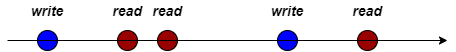
\includegraphics[scale=.5]{resources/memory_model_naive.png}
    \end{center}
    \begin{block}{Memory as a concurrent system}
        \begin{itemize}
            \item \alert{Operations}: $read, write$.
            \pause
            \item \alert{Semantics}: $read$ returns value of the last $write$.
        \end{itemize}    
    \end{block}
\end{frame}

\begin{frame}{Atomic Consistency: Jargon}
    \begin{center}
        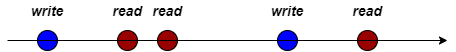
\includegraphics[scale=.5]{resources/memory_model_naive.png}
    \end{center}
    \begin{block}{Atomic Consistency a.k.a \textbf{Linearizability}}
        \begin{itemize}
            \item A strong \emph{Consistency Model}.
            \item Requires a \emph{total ordering} of operations.
            \item Requires operations be consistent with 'real timeline'.
        \end{itemize}
    \end{block}
\end{frame}
\begin{frame}
    \frametitle{Atomic Consistency - Auxilery Definitions}
    \begin{block}{Execution}
        An execution is a set of invocations to \emph{read} and \emph{write} operations,
        each is represented by an interval $[s,e]$ on
        the real number line where $s<e$.
    \end{block}
    \begin{center}
        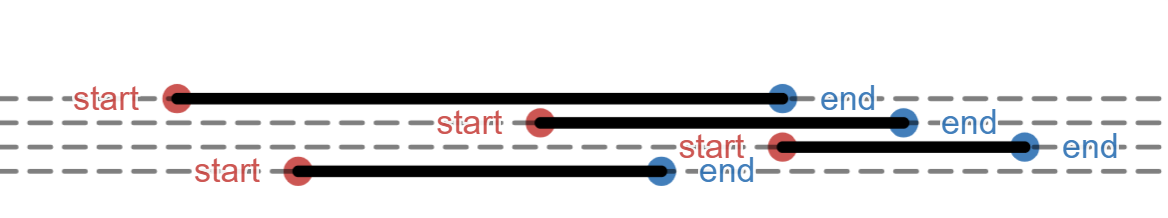
\includegraphics[scale=.5]{resources/execution_start_end.png}
    \end{center}
    \pause
    \begin{alertblock}{Serialization}
        Given an execution $[s_1, e_1], [s_2, e_2], ... [s_T, e_T]$,
        a serialization is unique set $a_1,a_2,...a_T$ s.t. $a_i\in[s_i,e_i]$.
    \end{alertblock}
    \begin{center}
        
\includegraphics[scale=.5]{resources/execution_serialization.png}
    \end{center}
\end{frame}
\begin{frame}
    \frametitle{Atomic Consistency - Auxilery Definitions}
    \textbf{Linearization = Serialization + Semantics}
    \pause
    \begin{alertblock}{Execution Linearizability}
        Execution is linearizable if exists a serialization which satisfies the system's semantics.
    \end{alertblock}
    % An execution $[s_1, e_1], [s_2, e_2], ... [s_T, e_T]$
    % is linearizable if there exists a serialization $a_1,...,a_T$ for it,
    % which consistent with the order of the operations, i.e.
    % if $a_i$ is a read operation, and $j=\max\{k\mid k<i\wedge a_k\text{ is write }\}$ (last write),
    % then $a_i$ returns the value written by $a_j$.
    \pause
    \begin{center}
        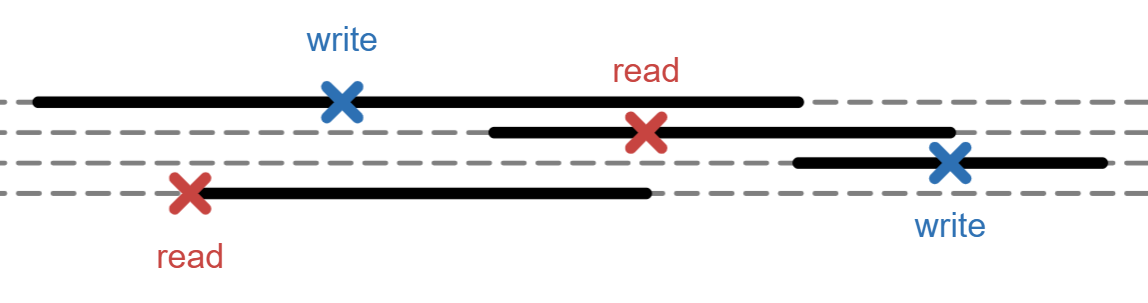
\includegraphics[scale=.35]{resources/linearization_x_1.png}
        \pause
        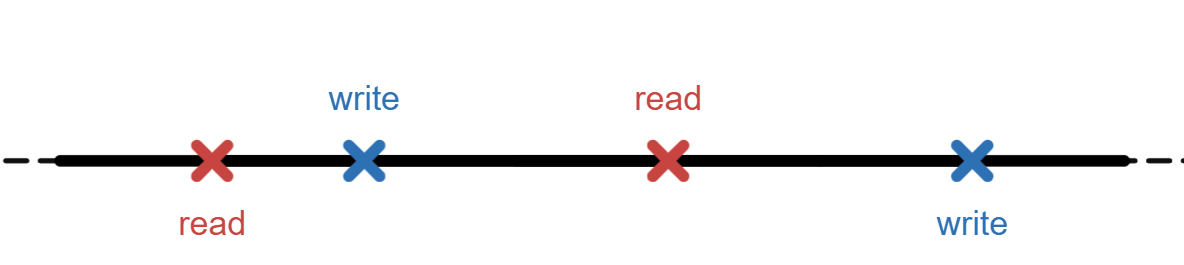
\includegraphics[scale=.35]{resources/linearization_x_2.png}
    \end{center}
    \pause
    \begin{block}{System Linearizability}
        System is linearizable if all possible executions are.
    \end{block}
\end{frame}
% \begin{frame}
%     \frametitle{Atomic Consistency}
%     \textbf{Atomic Consistency} a.k.a \textbf{Linearizability}.
%     \begin{block}{Definition}
%         \emph{'for any \alert{execution} of the system, there is some way of totally \alert{ordering}
%         the reads and writes so that the values returned by the reads are the same\\
%         \alert{as if the operations had been performed in that order}, with no overlap.'}\\
%         - 'On Interprocess Communication', Lamport (1985).
%     \end{block}
% \end{frame}
\begin{frame}
    \frametitle{Notations}
    We define these notations for any correct processes $p_i, p_j$:
    \begin{block}{Reads}
        $read[\alert{i,j,x}]$ will refer to an invocation by $p_i$, to read $Reg[\alert{j}]$
        which returns the \alert{$x$}'th value written by \alert{$p_j$}.
    \end{block}
    \begin{block}{Writes}
        $write[\alert{i,y}]$ will refer to the \alert{$y$}'th invocation by \alert{$p_i$}, to write $Reg[\alert{i}]$.
    \end{block}
    \pause
    Note: $read[i,j,x]$ does \textbf{NOT} mean the value $x$ was read,
    it means that the $x$'th value written to the register was read.\\
    Similarly with $write[i,y]$

\end{frame}
\begin{frame}
    \frametitle{Algorithm Correctness Requirments - Termination}
    Let $p_i$ be a correct process.
    \begin{block}{Write Termination}
        Each invocation of $Reg_i[i].write()$ terminates.
    \end{block}
    \begin{block}{Read Termination}
        For any $j$, all invocations $Reg_i[j].read()$ terminates.
    \end{block}
\end{frame}
\begin{frame}{Alternative Semantics}
    \begin{itemize}
        \item We want to require our algorithm to have atomic consistency.
        \pause
        \item That requires showing every read returns value of last write.
        \begin{center}
            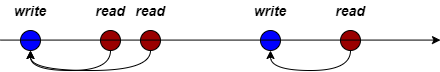
\includegraphics[scale=.4]{resources/vanilla_semantics.png}
        \end{center}
        \pause
        \item Instead we prove equivalent semantics - Read invocations should consistent with order of writes:
    \end{itemize}
    
\end{frame}

\begin{frame}{Algorithm Correctness Requirments - Atomic Consistency}
    For any correct $p_i, p_j, p_k$ where $p_i$ and $p_j$ are correct, require:
    \begin{block}{Write History Sequence}
        We can associate a single sequence $H_k[x]$ with $p_k$ with
        the set of writes by $p_k$ and 
        $H_k[x]$ is the value written by $write[k,x]$ if $p_k$ is correct.
    \end{block}
    \pause
    \begin{block}{Read followed by Write}
        if $read[j,i,x]$ terminates before $write[i,y]$ starts then $x<y$.
    \end{block}
    \pause
    \begin{block}{Write followed by Read}
        if $write[j,x]$ terminates before $read[i,j,y]$ starts then $x\leq y$.
    \end{block}
    \pause
    \begin{block}{No Read inversion}
        if $read[i,k,x]$ terminates before $read[j,k,y]$ starts then $x\leq y$.
    \end{block}    
\end{frame}

\begin{frame}
    \frametitle{Read Inversion - Example}
    $p_1$ reads before $p_2$, but gets
    an older value:
    \begin{center}
        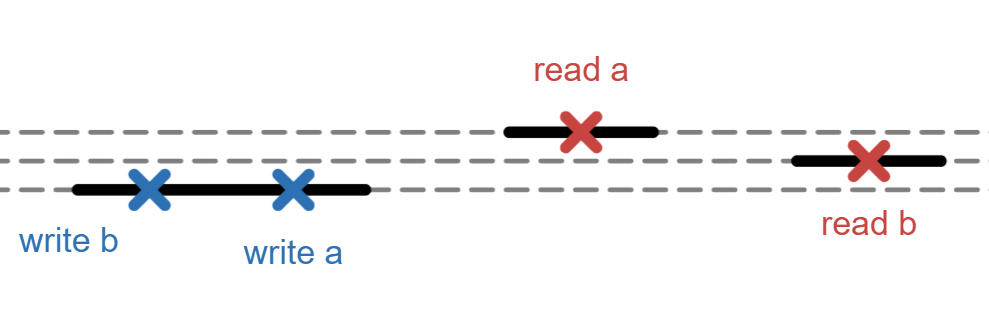
\includegraphics[scale=.6]{resources/read_inversion_lines.png}
    \end{center}
\end{frame}

% \begin{frame}
%     \frametitle{Linearization - A Visual Example}
%     \begin{center}
%         \href{https://www.desmos.com/calculator/v2ltnxcko2}{Demo}
%     \end{center}
% \end{frame}